\section{APPENDIX}

\subsection{Finger model data}
$F_0 = (123.0, 219.0, 23.52, 91.74,	21.6, 124.8, 129.6)$\\
$
JR = 
\begin{pmatrix}
-0.08941 & -0.0447 & -0.009249 & 0.03669 & 0.1421 & 0.2087 & -0.2138 \\
-0.04689 & -0.1496 & 0.052 &0.052 & 0.0248 & 0.0 & 0.0248 \\ 
0.06472 & 0.001953 & -0.1518 &-0.1518 & 0.2919 & 0.0568 & 0.2067 \\
0.003081 & -0.002352 & -0.0001649 & -0.0001649 & -0.0004483 & 0.0001578 & -0.000685
\end{pmatrix}$

$task_x = (1.0,0.0,0.0,0.0)$

$task_y = (0.0,1.0,0.0,0.0)$

Palmar force is $task_z = (0.0,0.0,1.0,0.0)$

%$task_xy = (1.0,1.0,0.0,0.0)$

\begin{figure}[h]
\centering
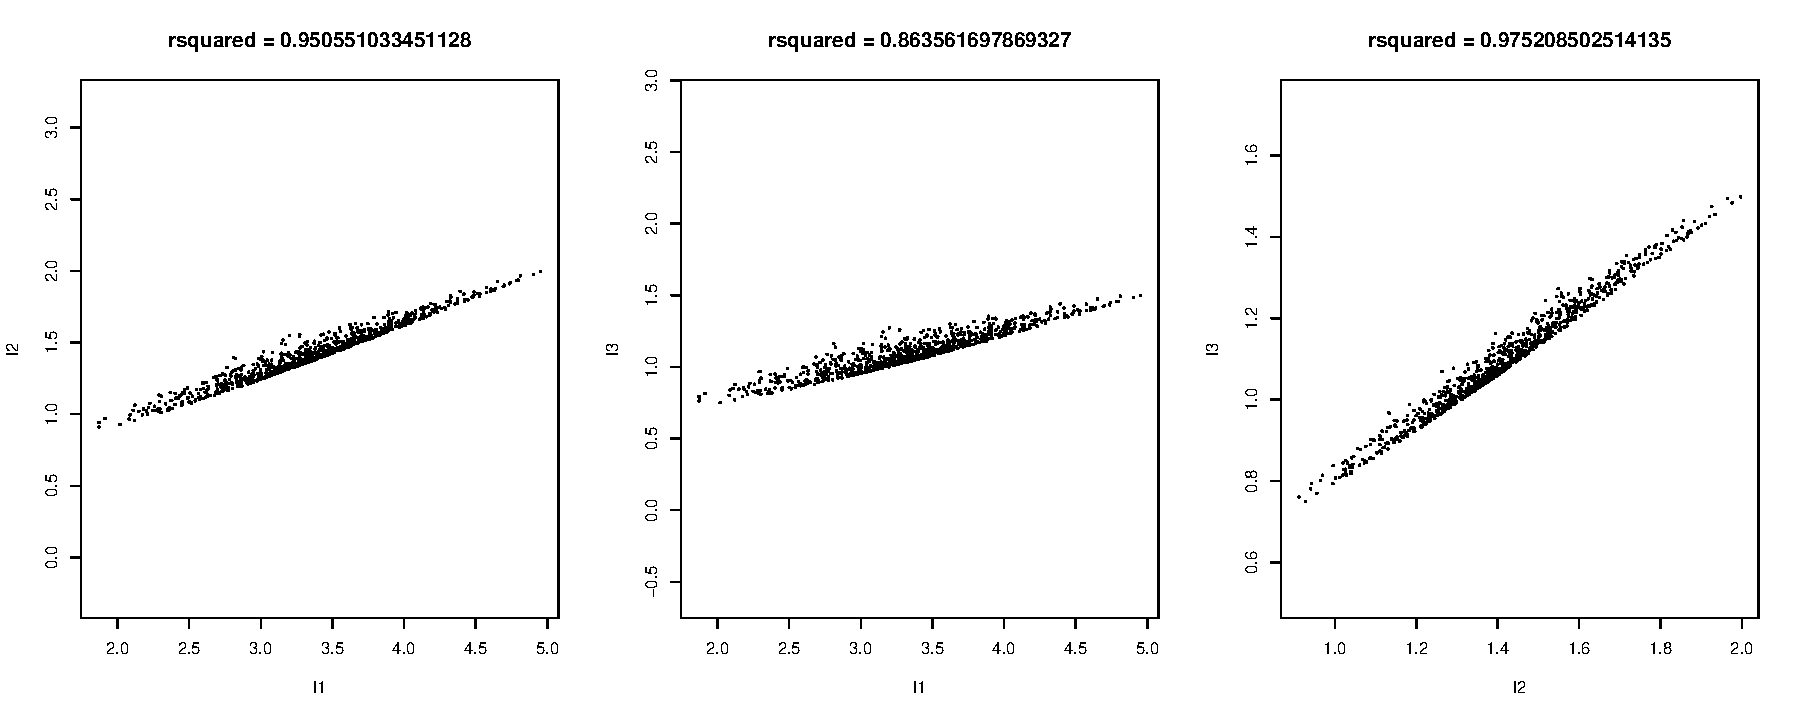
\includegraphics[width=\textwidth,page=1]{figs/cost_function_scatterplots.pdf}
\caption{Non weighted cost functions}
\label{fig:unweighted_cost_functions}
\end{figure}

\begin{figure}[h]
\centering
\includegraphics[width=\textwidth,page=2]{figs/cost_function_scatterplots.pdf}
\caption{Weighted cost functions}
\label{fig:weighted_cost_functions}
\end{figure}
The result of these computations (evaluated in R) shows the cumulative percentage of points up to each of those points.
\begin{verbatim}
# fixed_db database where each row is a point, each column is a muscle, and one column is the alpha level
library(stats)
eip_solutions <- fixed_db[fixed_db['alpha']==0.9,][,3]
activations_of_interest <- c(0.49,0.51)
ecdf(eip_solutions, activations_of_interest)
\end{verbatim}

We developed and tested our code in  Ubuntu 14.04, Windows 8.1, and OSX Yosemite 10.10.3; implemented Hit-and-Run with Scala 2.11.6\footnote{http://www.scala-lang.org/}, developed our histograms and descriptive statistics with R 3.1.3 \cite{rCoreCitation}, and designed our parallel coordinate visualization with multiple open-source JavaScript projects \footnote{http://syntagmatic.github.io/parallel-coordinates/}\footnote{http://d3js.org/}. All code and documentation used to develop this publication is readily available on a Github repository \footnote{https://github.com/bcohn12/space}
